\cleardoublepage


\chapter{Direkte Kinematik}\label{ch:direkte-kinematik}

Die direkte Kinematik ist dafür verantwortlich, aus den verschiedenen Winkeln und Positionen der Gelenke die Rotation und Position des Endeffektors im Raum zu berechnen.
Dazu wird zunächst in jedem Gelenk ein Koordinatenursprung gelegt, der eine Nullstellung jedes Gelenks beschreibt.
Um alle Gelenke in einer kinematischen Kette abzubilden, kann mit einem Parameter in den Freiheitsgraden des entsprechenden Gelenks eine Rechenvorschrift aufgebaut werden, um den Roboter zu beschreiben und die Position des Endeffektors schnell bestimmen zu können.

Zur Beschreibung von Transformationen wird in dieser Arbeit auf die Homogene Transformationsmatrix zurückgegriffen.
Diese besteht aus einer Rotationsmatrix $R_{a,b}$, die die Rotation von System $a$ in System $b$ beschreibt und einem Translationsvektor $P_{a,b}$, der die Translation zwischen den zwei Systemen entspricht~\ref{eq:inv-rule0}~\cite[28]{craigIntroductionRoboticsMechanics2009}.
Um eine Inverse Transformation von System $b$ in System $a$ zu erhalten, kann die Inverse der Transformationsmatrix $T_{a,b}$ oder die Regel aus Gleichung~\ref{eq:inv-rule1} verwendet werden.
Bei der Multiplikation zweier geeigneter Matrizen können mehrere Transformationen in einer Matrix dargestellt werden.
Ein Beispiel hierfür findet sich in Gleichung~\ref{eq:inv-rule2}.

\begin{equation}
    T_{a,b} = \begin{bmatrix}
                  R_{a,b} & P_{a,b} \\
                  0^T     & 1
    \end{bmatrix} \label{eq:inv-rule0}
\end{equation}
\begin{equation}
    T_{b,a} = \left( T_{a,b} \right)^{-1} =
    \begin{bmatrix}
        \left(R_{a,b}\right)^T & - \left(R_{a,b}\right)^T P_{a,b} \\
        0^T     & 1
    \end{bmatrix} =
    \begin{bmatrix}
        R_{b,a} & - R_{b,a}P_{a,b} \\
        0^T     & 1
    \end{bmatrix}
    \label{eq:inv-rule1}
\end{equation}
\begin{equation}
    T_{a,b}\cdot T_{b,c}=T_{a,c}    \label{eq:inv-rule2}
\end{equation}


\section{DH-Konvention}\label{sec:dh-konvention}

Um Rotation und Translation eines Gliedes der kinematischen Kette darzustellen kann die sog.\ DH-Konvention oder auch DH-Transformation verwendet werden.
Diese Konvention beschreibt ein standardisiertes Vorgehen wie die Transformation des nächsten Gelenks im Koordinatensystem des momentanen Gelenks ausgedrückt werden soll~\cite{denavitKinematicNotationLowerPair1955,craigIntroductionRoboticsMechanics2009}.
Es gelten die folgenden Regeln:

\begin{enumerate}
    \item Achse $z_{n}$ liegt entlang der Bewegungsachse des Gelenks $n$
    \item Achse $x_{n}$ liegt auf der kürzesten Verbindung zwischen Achsen $z_{n-1}$ und $z_{n}$.
    \item Die $y_{n}$ Achse wird rechtshändig ergänzt.
\end{enumerate}

Dabei sind die Ursprünge der Gelenkkordinatensysteme oftmals nicht im Gelenkursprung, was Komplexität für die Berechnung von Transformationen verringert.
Aus der Beziehung der zwei Koordinatensysteme können die DH-Parameter abgeleitet werden (siehe auch Abbildung~\ref{fig:dh-konvention1}):

\begin{itemize}
    \item $\theta_n$ Winkel zwischen $x_{n-1}$ und $x_n$ mit Rotationsachse $z_{n-1}$
    \item $d_n$: Kleinster Abstand zwischen $x_{n-1}$ und $x_n$
    \item $a_n$: Abstand zwischen den Achsen $z_{n-1}$ und $z_n$
    \item $\alpha_n$ Winkel zwischen $z_{n-1}$ und $z_n$ mit Rotationsachse $x_{n}$
\end{itemize}

Dies entspricht den folgenden Transformationsmatrizen (Gleichungen~\ref{eq:dh1},~\ref{eq:dh2},~\ref{eq:dh3},~\ref{eq:dh4}):

\newcommand{\ct}{\cos(\theta_n)}
\newcommand{\st}{\sin(\theta_n)}
\newcommand{\ca}{\cos(\alpha_n)}
\newcommand{\sa}{\sin(\alpha_n)}

\begin{equation}
    T_{\theta_n} =
    \begin{bmatrix}
        \ct & -\st & 0 & 0 \\
        \st & \ct  & 0 & 0 \\
        0   & 0    & 1 & 0 \\
        0   & 0    & 0 & 1 \\
    \end{bmatrix}
    \label{eq:dh1}
\end{equation}
\begin{equation}
    T_{d_n} =
    \begin{bmatrix}
        1 & 0 & 0 & 0   \\
        0 & 1 & 0 & 0   \\
        0 & 0 & 1 & d_n \\
        0 & 0 & 0 & 1   \\
    \end{bmatrix}
    \label{eq:dh2}
\end{equation}

\begin{equation}
    T_{a_n} =
    \begin{bmatrix}
        1 & 0 & 0 & a_n \\
        0 & 1 & 0 & 0   \\
        0 & 0 & 1 & 0   \\
        0 & 0 & 0 & 1   \\
    \end{bmatrix}
    \label{eq:dh3}
\end{equation}

\begin{equation}
    T_{\alpha_n} =
    \begin{bmatrix}
        1 & 0   & 0    & 0 \\
        0 & \ca & -\sa & 0 \\
        0 & \sa & \ca  & 0 \\
        0 & 0   & 0    & 1 \\
    \end{bmatrix}
    \label{eq:dh4}
\end{equation}

Um nun Koordinatensystem $n-1$ in Koordinatensystem $n$ zu überführen, kann die Transformationsmatrix $T_{n-1,n}$ verwendet werden (Gleichung~\ref{eq:dh5}).
Für den beweglichen Freiheitsgrad der Gelenke wird dann jeweils eine freie Variable festgelegt ($\theta_n$ für translatorische und $d_n$ für rotatorische Gelenke).

\begin{equation}
    T_{n-1,n}(\theta_n, d_n) \coloneqq T_{\theta_n} \cdot T_{d_n} \cdot T_{a_n} \cdot T_{\alpha_n} =
    \begin{bmatrix}
        \ct & -\st\ca & \st\sa  & a_n\ct \\
        \st & \ct\ca  & -\ct\sa & a_n\st \\
        0   & \sa     & \ca     & d_n    \\
        0   & 0       & 0       & 1      \\
    \end{bmatrix}
    \label{eq:dh5}
\end{equation}

\begin{figure}[h]
    \centering
    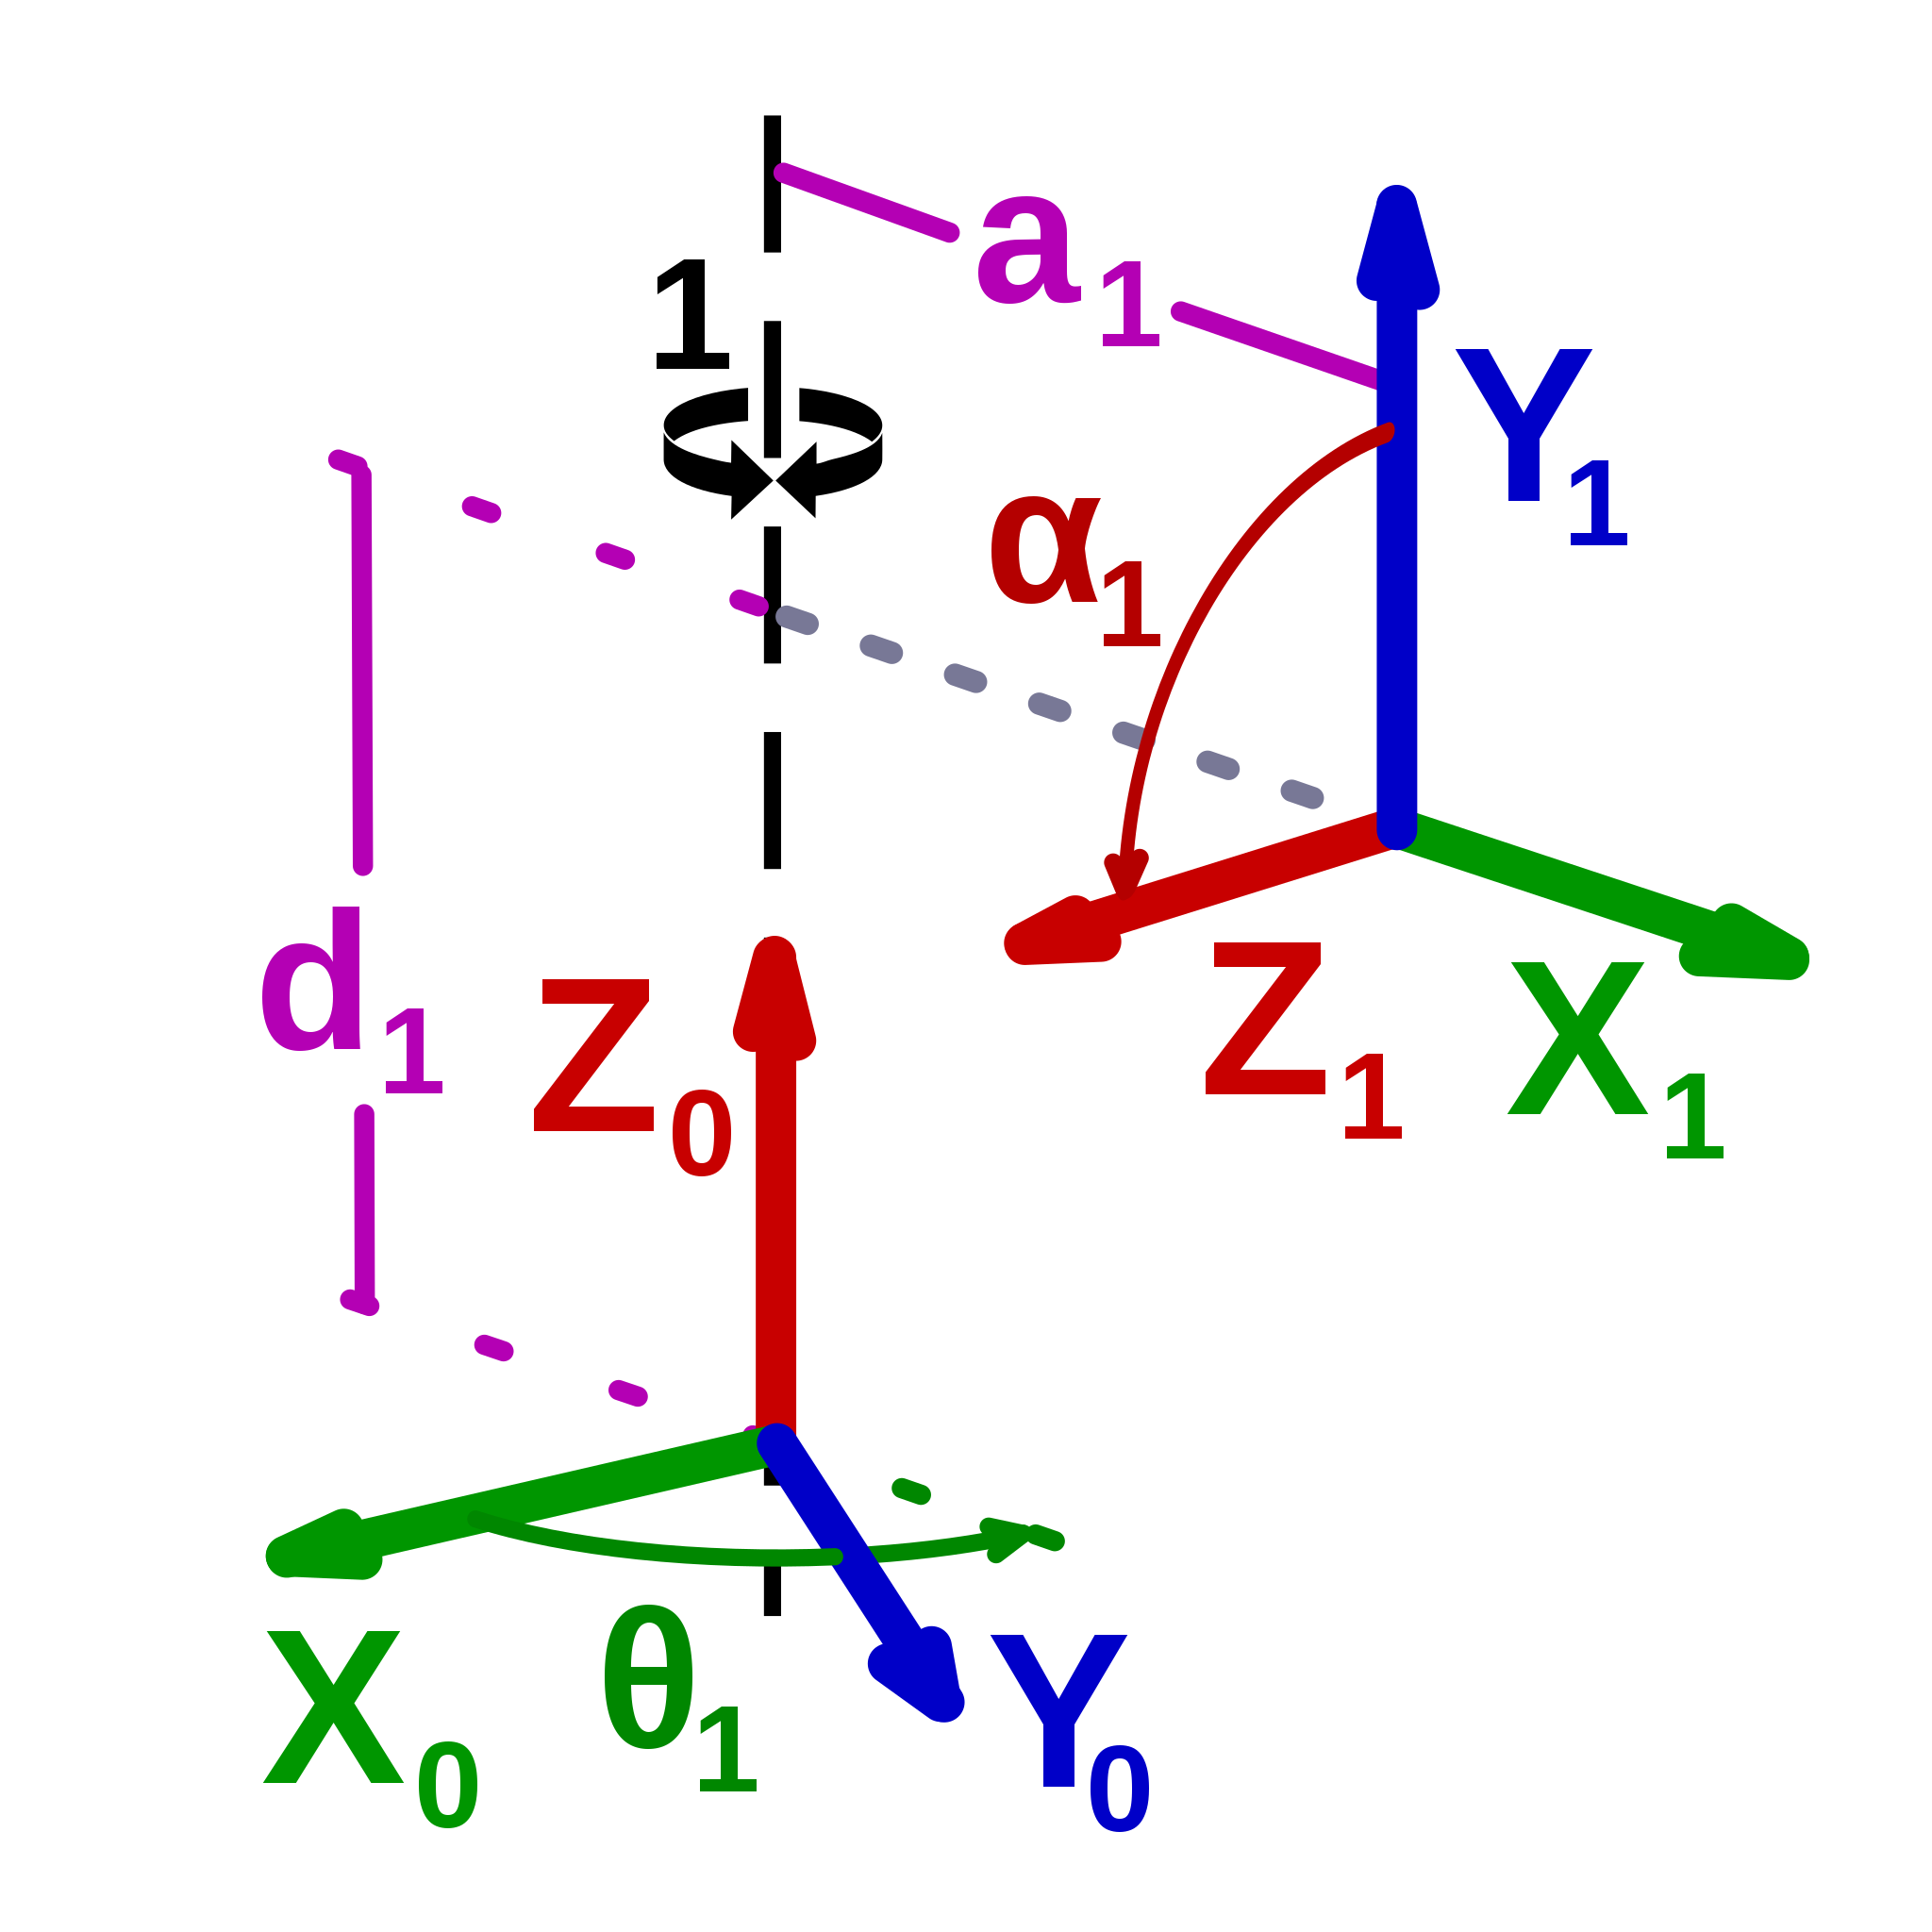
\includegraphics[width = .5\textwidth]{Bilder/Denavit-Hartenberg-Transformation.svg}
    \caption{DH-Konvention zwischen zwei Gelenken~\cite{jahobrCoordinateSystemsDenavitHartenberg2007}}\label{fig:dh-konvention1}
\end{figure}

Oftmals wird in der Literatur auch eine alternative, modifizierte Form der DH-Parameter verwendet~\cite[75]{craigIntroductionRoboticsMechanics2009}.
Um die Vergleichbarkeit mit~\cite{rasmusandersenKinematicsUR52018} zu gewährleisten wird in der Rechnung sowie im Code diese alternative Methode eingesetzt.
Dabei verändert sich die Transformationsmatrix eines Gelenks auf die Werte aus Gleichung~\ref{eq:alt-tf}:

\begin{equation}
    T_{n-1,n}(\theta_n, d_n) \coloneqq
    \begin{bmatrix}
        \ct                   & -\st                  & 0                   & a_{n-1}                  \\
        \st\cos(\alpha_{n-1}) & \ct\cos(\alpha_{n-1}) & -\sin(\alpha_{n-1}) & -d_{n}\sin(\alpha_{n-1}) \\
        \st\sin(\alpha_{n-1}) & \ct\sin(\alpha_{n-1}) & \cos(\alpha_{n-1})  & d_{n}\cos(\alpha_{n-1})  \\
        0                     & 0                     & 0                   & 1                        \\
    \end{bmatrix}
    \label{eq:alt-tf}
\end{equation}


\section{Unified Robot Description Format}\label{sec:urdf}

Das \ac{urdf} ist ein Standard, entwickelt für \ac{ros}, der sowohl die geometrischen als auch physischen und visuellen Eigenschaften eines Roboters beschreiben kann.
Dafür ist eine auf XML basierende Datei nötig, die mithilfe von XML-Tags den Roboter aus sog. \enquote{Links} und \enquote{Joints} aufbaut~\cite{ros.orgUrdfXMLModel}.

Links sind die physischen Verbindungen zwischen zwei Gelenken und können verschiedene Eigenschaften aufweisen.
Neben den dem geometrischen Aufbau wird zudem unterschieden zwischen visuellen Eigenschaften (\enquote{visual}), Kollisionseigenschaften (\enquote{collision}) und Trägheitseigenschaften (\enquote{inertial}).

Joints sind Gelenke, die aus der Verbindung zweier physischer Links bestehen.
Dabei sind nicht nur translatorische (\enquote{prismatic}) und rotatorische Gelenke (\enquote{revolute}) beschreibbar, sondern auch feste (\enquote{fixed}), schwebende (\enquote{floating}) und planare Verbindungen (\enquote{planar}).
Für die Beschreibung eines Joints wird der vorhergehende Link als \enquote{parent} und der nächste Link als \enquote{child} bezeichnet.
Zudem müssen im Feld \enquote{origin} Translation und Rotation des Ursprungs im Koordinatensystem des Parent Links, sowie im Feld \enquote{axis} je nach Gelenk die Rotationsachse, Translationsachse oder Normale der Bewegungsoberfläche angegeben werden.
Desweiteren ist es möglich, Schnittstellen für die Bewegung der Motoren zu definieren und Bewegungslimits für die Gelenke anzugeben, um die Ansteuerung des Roboters und die Bewegungsplanung zu vereinfachen.

Die Schritte zur Berechnung der direkten Kinematik können für das bessere Verständnis im Code ?? (Anhang referenz) direkt nachvollzogen und visualisiert werden.


\section{Beschreibung des UR5}\label{sec:ur5-in-dh}
Der in dieser Arbeit betrachtete Roboter ist der UR5e von Universal Robots.
Dieser ist ein vergleichsweise günstiger Roboter mit verringerter Zahl an Singularitäten (siehe Abschnitt~\ref{sec:singularitaten}), sechs Gelenken und einer offenen kinematischen Kette.
Offiziell wird der Roboter mit den DH-Parametern aus Tabelle~\ref{tab:ur5-dh1} und dynamischen Eigenschaften der Links aus Tabelle~\ref{tab:ur5-dh2} beschrieben~\cite{universalrobotsUniversalRobotsDH}.
Abbildung~\ref{fig:ur5-axis} kann zudem die Dimensionierung des Roboters und die Anordnung der Achsen in Nullstellung entnommen werden.

Nach Datenblatt~\cite{universalrobotsUR5TechnicalSpecifications} hat der UR5 einen Arbeitsraum mit Radius 85cm (Abstand vom Befestigungspunkt bei ausgestrecktem Arm) und kann sich mit einer Maximalgeschwindigkeit von bis zu 180°/s bewegen.

\begin{figure}[h]
    \centering
    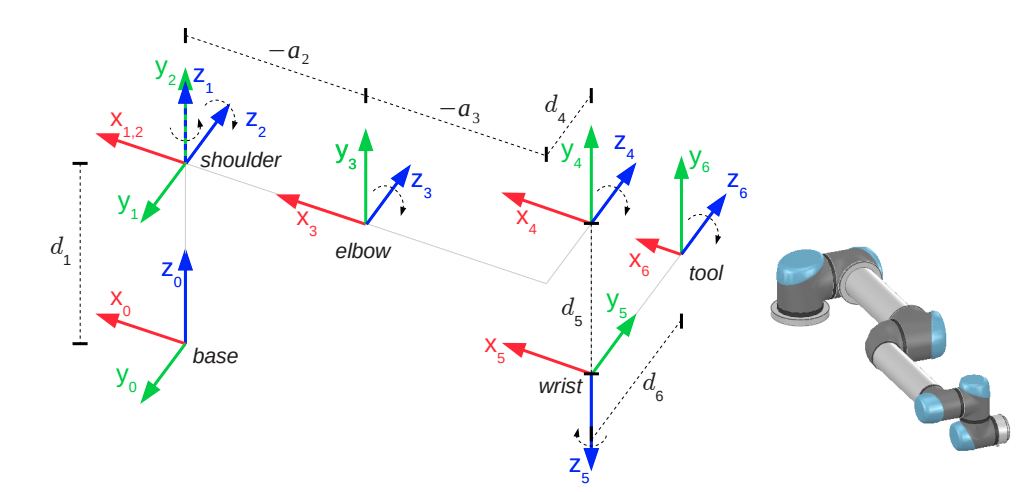
\includegraphics[width = .9\textwidth]{Bilder/ur5-axis}
    \caption{Achsen des UR5-Roboters mit Angabe der DH-Parameter (links) und Visualisierung der Nullposition (rechts)~\cite{rasmusandersenKinematicsUR52018}}\label{fig:ur5-axis}
\end{figure}

\begin{table}
    \centering
    \begin{tabular}{lrrrllrl}
        \toprule
        \textbf{Joint} & $\boldsymbol{\theta}$ \textbf{[rad]} & $\boldsymbol{a}$ \textbf{[m]} & $\boldsymbol{d}$ \textbf{[m]} & $\boldsymbol{\alpha}$ \textbf{[rad]}  \\
        \midrule
        Joint 1        & 0                                    & 0                             & 0.089159                      & \pi/2                                \\
        Joint 2        & 0                                    & -0.425                        & 0                             & 0                                    \\
        Joint 3        & 0                                    & -0.3922                       & 0                             & 0                                    \\
        Joint 4        & 0                                    & 0                             & 0.10915                       & \pi/2                                \\
        Joint 5        & 0                                    & 0                             & 0.09465                       & -\pi/2                               \\
        Joint 6        & 0                                    & 0                             & 0.0823                        & 0                                    \\
        \bottomrule
    \end{tabular}
    \caption{DH-Parameter des UR5e Roboters von Universal Robots~\cite{universalrobotsUniversalRobotsDH}}
    \label{tab:ur5-dh1}
\end{table}
\begin{table}
    \centering
    \begin{tabular}{lrrrllrl}
        \toprule
        \textbf{Link} & \textbf{Masse [kg]} & \textbf{Schwerpunkt [m]} \\
        \midrule
        Link 1        & 3.7                 & [0, -0.02561, 0.00193]   \\
        Link 2        & 8.393               & [0.2125, 0, 0.11336]     \\
        Link 3        & 2.33                & [0.15, 0.0, 0.0265]      \\
        Link 4        & 1.219               & [0, -0.0018, 0.01634]    \\
        Link 5        & 1.219               & [0, 0.0018,0.01634]      \\
        Link 6        & 0.1879              & [0, 0, -0.001159]        \\
        \bottomrule
    \end{tabular}
    \caption{Beschreibung der dynamischen Eigenschaften des UR5e Roboters von Universal Robots~\cite{universalrobotsUniversalRobotsDH}}
    \label{tab:ur5-dh2}
\end{table}


\section{Geschwindigkeitskinematik}\label{sec:geschwindigkeitskinematik}

Um einen Roboter in Bewegung darzustellen, ist nicht nur die Transformation der Gelenke relevant, sondern auch dessen Kinematik und Dynamik.
Dies ist besonders relevant, da in der echten Welt bestimmte Maximalwerte für (Winkel-) Geschwindigkeit und Beschleunigung, sowie Trägheit und Drehmoment eingehalten werden müssen, um den sicheren Betrieb sowie das Verhalten der Masse korrekt abzubilden.

Für die Berechnung der Geschwindigkeit des Endeffektors im Gelenk $e$ kann die Jakobi-Matrix verwendet werden~\cite[105ff]{sicilianoRobotics2009}.
Dabei gilt für eine Drehung nach DH-Konvention um Achse $z_{n-1}$ für die Geschwindigkeit Gleichung~\ref{eq:kin-1} und für die Winkelgeschwindigkeit Gleichung~\ref{eq:kin-2}.
Für translatorische Gelenke gelten stattdessen Gleichungen~\ref{eq:kin-1-1} und~\ref{eq:kin-2-1}.
Die Vektoren $z_{i}$ entsprechen jeweils der Einheitsvektor der z-Achse $z_{i} = \frac{Z_{0,i}}{\lvert Z_{0,i} \rvert}$ auf Basis der Transformationsmatrix $T_{0,i} = \prod_{n=1}^{i}T_{n-1,n}$ (siehe Konvention Gleichung~\ref{eq:inv-konv}).

\begin{equation}
    J_{P_{n}} = z_{n-1} \times (P_{e} - P_{n-1}) \label{eq:kin-1}
\end{equation}
\begin{equation}
    J_{\omega_{n+1}} = z_{n-1} \label{eq:kin-2}
\end{equation}
\begin{equation}
    J_{P_{n}} = z_{n-1} \label{eq:kin-1-1}
\end{equation}
\begin{equation}
    J_{\omega_{n+1}} = 0 \label{eq:kin-2-1}
\end{equation}

Für alle Gelenke ergibt sich dann für die Jakobi-Matrix eines Sechs-Achsen-Roboters wie dem UR5 die folgende Gleichung~\ref{eq:kin-3} mit jeweils sechs Spalten und Zeilen.
Um die Geschwindigkeit des Endeffektors $v_6$ zu erhalten, muss die Matrix mit der Geschwindigkeit $\dot{\theta}$ multipliziert werden (Gleichung~~\ref{eq:kin-4}).

\begin{equation}
    J_{0,6}=
    \begin{pmatrix}
        J_{P_1}      & \dots & J_{P_6}      \\
        J_{\omega_1} & \dots & J_{\omega_6}
    \end{pmatrix}\label{eq:kin-3}
\end{equation}
\begin{equation}
    v_6 =
    \begin{pmatrix}
        \dot{P}_{0,6} \\ \omega_6
    \end{pmatrix} =
    J_{0,6}\cdot\dot{\theta}
    \label{eq:kin-4}
\end{equation}